\documentclass[aspectratio=169]{beamer}
\usetheme{Madrid}
\usecolortheme{default}
\setbeamertemplate{caption}{\raggedright\insertcaption\par}
\usepackage{fontspec}
\usepackage{graphicx}
\usepackage{hyperref}
\usepackage{booktabs}
\usepackage{xcolor}
\usepackage{listings}

\lstset{
    language=Python,
    basicstyle=\ttfamily\small,
    keywordstyle=\color{blue},
    stringstyle=\color{red},
    commentstyle=\color{green!50!black},
    showstringspaces=false,
    breaklines=true,
    frame=single,
    backgroundcolor=\color{gray!10}
}

\title[Thực hành Chương 1]{THỰC HÀNH: TỔNG QUAN HỌC MÁY \\ \vspace{0.5cm} \Large Hướng dẫn chi tiết}
\author{TS. Trần Thành Thắng}
\institute{Đại học Đông Á}
\date{\today}

\begin{document}

\begin{frame}[allowframebreaks]{Hướng dẫn thực hành}
Chương 1 - Bối cảnh máy học



\_Sổ tay này chứa các ví dụ về mã ở chương 1. Bạn cũng sẽ tìm thấy lời giải bài tập ở cuối sổ tay. Phần còn lại của sổ ghi chép này được sử dụng để tạo lifesat.csv từ các nguồn dữ liệu gốc và một số số liệu của chương này.\_



Bạn có thể xem qua mã trong sổ tay này nếu muốn, nhưng hành động thực sự sẽ bắt đầu ở chương tiếp theo.


\end{frame}

\begin{frame}[allowframebreaks]{Cài đặt}


  

    

  

  

    

  



\# Cài đặt

Dự án này yêu cầu Python 3.7 trở lên:


\end{frame}

\begin{frame}[fragile]{Cài đặt (Tiếp theo 1)}
\begin{lstlisting}[language=Python]
import sys

assert sys.version_info >= (3, 7)
\end{lstlisting}

Scikit-Learn ≥1.0.1 là bắt buộc:

\begin{lstlisting}[language=Python]
from packaging import version
import sklearn

assert version.parse(sklearn.__version__) >= version.parse("1.0.1")
\end{lstlisting}

Hãy xác định kích thước phông chữ mặc định để vẽ các hình vẽ đẹp:


\end{frame}

\begin{frame}[fragile]{Cài đặt (Tiếp theo 2)}
\begin{lstlisting}[language=Python]
import matplotlib.pyplot as plt

plt.rc('font', size=12)
plt.rc('axes', labelsize=14, titlesize=14)
plt.rc('legend', fontsize=12)
plt.rc('xtick', labelsize=10)
plt.rc('ytick', labelsize=10)
\end{lstlisting}

Làm cho đầu ra của sổ ghi chép này ổn định trong các lần chạy:


\end{frame}

\begin{frame}[fragile]{Cài đặt (Tiếp theo 3)}
\begin{lstlisting}[language=Python]
import numpy as np

np.random.seed(42)
\end{lstlisting}


\end{frame}

\begin{frame}[allowframebreaks]{Mã ví dụ 1-1}
\# Mã ví dụ 1-1


\end{frame}

\begin{frame}[fragile]{Mã ví dụ 1-1 (Tiếp theo 1)}
\begin{lstlisting}[language=Python]
import matplotlib.pyplot as plt
import numpy as np
import pandas as pd
from sklearn.linear_model import LinearRegression

# Download and prepare the data
data_root = "https://github.com/ageron/data/raw/main/"
lifesat = pd.read_csv(data_root + "lifesat/lifesat.csv")
X = lifesat[["GDP per capita (USD)"]].values
y = lifesat[["Life satisfaction"]].values

# Visualize the data
lifesat.plot(kind='scatter', grid=True,
             x="GDP per capita (USD)", y="Life satisfaction")
\end{lstlisting}


\end{frame}

\begin{frame}[fragile]{Mã ví dụ 1-1 (Tiếp theo 2)}
\begin{lstlisting}[language=Python]
plt.axis([23_500, 62_500, 4, 9])
plt.show()

# Select a linear model
model = LinearRegression()

# Train the model
model.fit(X, y)

# Make a prediction for Cyprus
X_new = [[37_655.2]]  # Cyprus' GDP per capita in 2020
print(model.predict(X_new)) # outputs [[6.30165767]]
\end{lstlisting}


\end{frame}

\begin{frame}[allowframebreaks]{Mã ví dụ 1-1 (Biểu đồ)}
\begin{center}
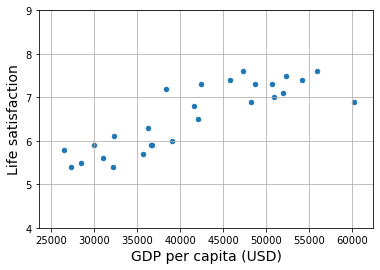
\includegraphics[width=\textwidth,height=0.75\textheight,keepaspectratio]{images/ch01/cell_12_out_0.png}
\end{center}


\end{frame}

\begin{frame}[fragile]{Mã ví dụ 1-1 (Biểu đồ) (Tiếp theo 1)}
\textbf{Kết quả:}
\begin{verbatim}
[[6.30165767]]
\end{verbatim}


\end{frame}

\begin{frame}[allowframebreaks]{Mã ví dụ 1-1 (Biểu đồ)}
Việc thay thế mô hình hồi quy tuyến tính bằng hồi quy k-Láng giềng gần nhất (trong ví dụ này là k = 3) trong mã trước đó cũng đơn giản như việc thay thế hai mô hình này

dòng:



 python

from sklearn.linear\_model import LinearRegression



model = LinearRegression()

  



with these two:



  python

from sklearn.neighbors import KNeighborsRegressor



model = KNeighborsRegressor(n\_neighbors=3)

 


\end{frame}

\begin{frame}[fragile]{Mã ví dụ 1-1 (Biểu đồ) (Tiếp theo 3)}
\begin{lstlisting}[language=Python]
# Select a 3-Nearest Neighbors regression model
from sklearn.neighbors import KNeighborsRegressor

model = KNeighborsRegressor(n_neighbors=3)

# Train the model
model.fit(X, y)

# Make a prediction for Cyprus
print(model.predict(X_new)) # outputs [[6.33333333]]
\end{lstlisting}


\end{frame}

\begin{frame}[fragile]{Mã ví dụ 1-1 (Biểu đồ) (Tiếp theo 4)}
\textbf{Kết quả:}
\begin{verbatim}
[[6.33333333]]
\end{verbatim}


\end{frame}

\begin{frame}[allowframebreaks]{Tạo dữ liệu và số liệu - vui lòng bỏ qua}
\# Tạo dữ liệu và số liệu - vui lòng bỏ qua

Đây là mã tôi đã sử dụng để tạo tập dữ liệu lifesat.csv. Bạn có thể bỏ qua điều này một cách an toàn.

Tạo hàm để lưu số liệu:


\end{frame}

\begin{frame}[fragile]{Tạo dữ liệu và số liệu - vui lòng bỏ qua (Tiếp theo 1)}
\begin{lstlisting}[language=Python]
from pathlib import Path

# Where to save the figures
IMAGES_PATH = Path() / "images" / "fundamentals"
IMAGES_PATH.mkdir(parents=True, exist_ok=True)

def save_fig(fig_id, tight_layout=True, fig_extension="png", resolution=300):
    path = IMAGES_PATH / f"{fig_id}.{fig_extension}"
    if tight_layout:
        plt.tight_layout()
    plt.savefig(path, format=fig_extension, dpi=resolution)
\end{lstlisting}


\end{frame}

\begin{frame}[allowframebreaks]{Tải và chuẩn bị dữ liệu Sự hài lòng trong cuộc sống}
\#\# Tải và chuẩn bị dữ liệu Sự hài lòng trong cuộc sống

Để tạo lifesat.csv , tôi đã tải xuống dữ liệu Chỉ số cuộc sống tốt hơn (BLI) từ trang web của OECD (để lấy Chỉ số hài lòng về cuộc sống cho từng quốc gia) và dữ liệu GDP bình quân đầu người của Ngân hàng Thế giới từ OurWorldInData.org. Dữ liệu BLI ở datasets/lifesat/oecd\_bli.csv (dữ liệu từ năm 2020) và dữ liệu GDP bình quân đầu người ở datasets/lifesat/gdp\_per\_capita.csv (dữ liệu đến năm 2020).



Nếu bạn muốn lấy các phiên bản mới nhất, xin vui lòng làm như vậy. Tuy nhiên, có thể có một số thay đổi (ví dụ: trong tên cột hoặc các quốc gia khác bị thiếu dữ liệu), vì vậy hãy chuẩn bị tinh chỉnh mã.


\end{frame}

\begin{frame}[fragile]{Tải và chuẩn bị dữ liệu Sự hài lòng trong cuộc sống (Tiếp theo 1)}
\begin{lstlisting}[language=Python]
import urllib.request

datapath = Path() / "datasets" / "lifesat"
datapath.mkdir(parents=True, exist_ok=True)

data_root = "https://github.com/ageron/data/raw/main/"
for filename in ("oecd_bli.csv", "gdp_per_capita.csv"):
    if not (datapath / filename).is_file():
        print("Downloading", filename)
        url = data_root + "lifesat/" + filename
        urllib.request.urlretrieve(url, datapath / filename)
\end{lstlisting}


\end{frame}

\begin{frame}[fragile]{Tải và chuẩn bị dữ liệu Sự hài lòng trong cuộc sống (Tiếp theo 2)}
\textbf{Kết quả:}
\begin{verbatim}
Downloading oecd_bli.csv
Downloading gdp_per_capita.csv
\end{verbatim}

\begin{lstlisting}[language=Python]
oecd_bli = pd.read_csv(datapath / "oecd_bli.csv")
gdp_per_capita = pd.read_csv(datapath / "gdp_per_capita.csv")
\end{lstlisting}

Xử lý trước dữ liệu GDP bình quân đầu người để chỉ giữ lại năm 2020:


\end{frame}

\begin{frame}[fragile]{Tải và chuẩn bị dữ liệu Sự hài lòng trong cuộc sống (Tiếp theo 3)}
\begin{lstlisting}[language=Python]
gdp_year = 2020
gdppc_col = "GDP per capita (USD)"
lifesat_col = "Life satisfaction"

gdp_per_capita = gdp_per_capita[gdp_per_capita["Year"] == gdp_year]
gdp_per_capita = gdp_per_capita.drop(["Code", "Year"], axis=1)
gdp_per_capita.columns = ["Country", gdppc_col]
gdp_per_capita.set_index("Country", inplace=True)

gdp_per_capita.head()
\end{lstlisting}


\end{frame}

\begin{frame}[fragile]{Tải và chuẩn bị dữ liệu Sự hài lòng trong cuộc sống (Tiếp theo 4)}
\textbf{Kết quả:}
\begin{verbatim}
GDP per capita (USD)
Country                                          
Afghanistan                           1978.961579
Africa Eastern and Southern           3387.594670
Africa Western and Central            4003.158913
Albania                              13295.410885
Algeria                              10681.679297
\end{verbatim}

Xử lý trước dữ liệu OECD BLI để chỉ giữ lại cột Life satisfaction:


\end{frame}

\begin{frame}[fragile]{Tải và chuẩn bị dữ liệu Sự hài lòng trong cuộc sống (Tiếp theo 5)}
\begin{lstlisting}[language=Python]
oecd_bli = oecd_bli[oecd_bli["INEQUALITY"]=="TOT"]
oecd_bli = oecd_bli.pivot(index="Country", columns="Indicator", values="Value")

oecd_bli.head()
\end{lstlisting}


\end{frame}

\begin{frame}[fragile]{Tải và chuẩn bị dữ liệu Sự hài lòng trong cuộc sống (Tiếp theo 6)}
\textbf{Kết quả:}
\begin{verbatim}
Indicator  Air pollution  Dwellings without basic facilities  \
Country                                                        
Australia            5.0                                 NaN   
Austria             16.0                                 0.9   
Belgium             15.0                                 1.9   
Brazil              10.0                                 6.7   
Canada               7.0                                 0.2   

Indicator  Educational attainment  Employees working very long hours  \
Country                                                                
Australia                    81.0                              13.04   
Austria                      85.0                               6.66   
Belgium                      77.0                               4.75   
Brazil                       49.0                               7.13   
Canada                       91.0                               3.69   
... (đã cắt bớt)
\end{verbatim}


\end{frame}

\begin{frame}[fragile]{Tải và chuẩn bị dữ liệu Sự hài lòng trong cuộc sống (Tiếp theo 7)}
Bây giờ, hãy hợp nhất dữ liệu về mức độ hài lòng với cuộc sống và dữ liệu GDP bình quân đầu người, chỉ giữ lại các cột GDP bình quân đầu người và mức độ hài lòng với cuộc sống:

\begin{lstlisting}[language=Python]
full_country_stats = pd.merge(left=oecd_bli, right=gdp_per_capita,
                              left_index=True, right_index=True)
full_country_stats.sort_values(by=gdppc_col, inplace=True)
full_country_stats = full_country_stats[[gdppc_col, lifesat_col]]

full_country_stats.head()
\end{lstlisting}


\end{frame}

\begin{frame}[fragile]{Tải và chuẩn bị dữ liệu Sự hài lòng trong cuộc sống (Tiếp theo 8)}
\textbf{Kết quả:}
\begin{verbatim}
GDP per capita (USD)  Life satisfaction
Country                                              
South Africa          11466.189672                4.7
Colombia              13441.492952                6.3
Brazil                14063.982505                6.4
Mexico                17887.750736                6.5
Chile                 23324.524751                6.5
\end{verbatim}


\end{frame}

\begin{frame}[fragile]{Tải và chuẩn bị dữ liệu Sự hài lòng trong cuộc sống (Tiếp theo 9)}
Để minh họa nguy cơ điều chỉnh quá mức, tôi chỉ sử dụng một phần dữ liệu trong hầu hết các số liệu (tất cả các quốc gia có GDP bình quân đầu người trong khoảng min\_gdp đến max\_gdp ). Ở phần sau của chương này, tôi sẽ tiết lộ những quốc gia còn thiếu và chỉ ra rằng chúng không theo cùng một xu hướng tuyến tính nào cả.

\begin{lstlisting}[language=Python]
min_gdp = 23_500
max_gdp = 62_500

country_stats = full_country_stats[(full_country_stats[gdppc_col] >= min_gdp) &
                                   (full_country_stats[gdppc_col] <= max_gdp)]
country_stats.head()
\end{lstlisting}


\end{frame}

\begin{frame}[fragile]{Tải và chuẩn bị dữ liệu Sự hài lòng trong cuộc sống (Tiếp theo 10)}
\textbf{Kết quả:}
\begin{verbatim}
GDP per capita (USD)  Life satisfaction
Country                                         
Russia           26456.387938                5.8
Greece           27287.083401                5.4
Turkey           28384.987785                5.5
Latvia           29932.493910                5.9
Hungary          31007.768407                5.6
\end{verbatim}

\begin{lstlisting}[language=Python]
country_stats.to_csv(datapath / "lifesat.csv")
full_country_stats.to_csv(datapath / "lifesat_full.csv")
\end{lstlisting}


\end{frame}

\begin{frame}[fragile]{Tải và chuẩn bị dữ liệu Sự hài lòng trong cuộc sống (Tiếp theo 11)}
\begin{lstlisting}[language=Python]
country_stats.plot(kind='scatter', figsize=(5, 3), grid=True,
                   x=gdppc_col, y=lifesat_col)

min_life_sat = 4
max_life_sat = 9

position_text = {
    "Turkey": (29_500, 4.2),
    "Hungary": (28_000, 6.9),
    "France": (40_000, 5),
    "New Zealand": (28_000, 8.2),
    "Australia": (50_000, 5.5),
    "United States": (59_000, 5.3),
    "Denmark": (46_000, 8.5)
\end{lstlisting}


\end{frame}

\begin{frame}[fragile]{Tải và chuẩn bị dữ liệu Sự hài lòng trong cuộc sống (Tiếp theo 12)}
\begin{lstlisting}[language=Python]
}

for country, pos_text in position_text.items():
    pos_data_x = country_stats[gdppc_col].loc[country]
    pos_data_y = country_stats[lifesat_col].loc[country]
    country = "U.S." if country == "United States" else country
    plt.annotate(country, xy=(pos_data_x, pos_data_y),
                 xytext=pos_text, fontsize=12,
                 arrowprops=dict(facecolor='black', width=0.5,
                                 shrink=0.08, headwidth=5))
    plt.plot(pos_data_x, pos_data_y, "ro")

plt.axis([min_gdp, max_gdp, min_life_sat, max_life_sat])

\end{lstlisting}


\end{frame}

\begin{frame}[fragile]{Tải và chuẩn bị dữ liệu Sự hài lòng trong cuộc sống (Tiếp theo 13)}
\begin{lstlisting}[language=Python]
save_fig('money_happy_scatterplot')
plt.show()
\end{lstlisting}


\end{frame}

\begin{frame}[allowframebreaks]{Tải và chuẩn bị dữ liệu Sự hài lòng trong cuộc sống (Biểu đồ)}
\begin{center}
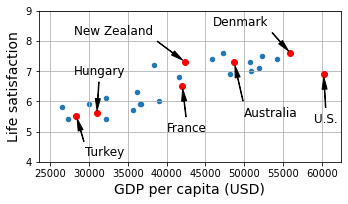
\includegraphics[width=\textwidth,height=0.75\textheight,keepaspectratio]{images/ch01/cell_32_out_0.png}
\end{center}


\end{frame}

\begin{frame}[fragile]{Tải và chuẩn bị dữ liệu Sự hài lòng trong cuộc sống (Biểu đồ) (Tiếp theo 1)}
\begin{lstlisting}[language=Python]
highlighted_countries = country_stats.loc[list(position_text.keys())]
highlighted_countries[[gdppc_col, lifesat_col]].sort_values(by=gdppc_col)
\end{lstlisting}


\end{frame}

\begin{frame}[fragile]{Tải và chuẩn bị dữ liệu Sự hài lòng trong cuộc sống (Biểu đồ) (Tiếp theo 2)}
\textbf{Kết quả:}
\begin{verbatim}
GDP per capita (USD)  Life satisfaction
Country                                               
Turkey                 28384.987785                5.5
Hungary                31007.768407                5.6
France                 42025.617373                6.5
New Zealand            42404.393738                7.3
Australia              48697.837028                7.3
Denmark                55938.212809                7.6
United States          60235.728492                6.9
\end{verbatim}


\end{frame}

\begin{frame}[fragile]{Tải và chuẩn bị dữ liệu Sự hài lòng trong cuộc sống (Biểu đồ) (Tiếp theo 3)}
\begin{lstlisting}[language=Python]
country_stats.plot(kind='scatter', figsize=(5, 3), grid=True,
                   x=gdppc_col, y=lifesat_col)

X = np.linspace(min_gdp, max_gdp, 1000)

w1, w2 = 4.2, 0
plt.plot(X, w1 + w2 * 1e-5 * X, "r")
plt.text(40_000, 4.9, fr"$\theta_0 = {w1}$", color="r")
plt.text(40_000, 4.4, fr"$\theta_1 = {w2}$", color="r")

w1, w2 = 10, -9
plt.plot(X, w1 + w2 * 1e-5 * X, "g")
plt.text(26_000, 8.5, fr"$\theta_0 = {w1}$", color="g")
plt.text(26_000, 8.0, fr"$\theta_1 = {w2} \times 10^{{-5}}$", color="g")
\end{lstlisting}


\end{frame}

\begin{frame}[fragile]{Tải và chuẩn bị dữ liệu Sự hài lòng trong cuộc sống (Biểu đồ) (Tiếp theo 4)}
\begin{lstlisting}[language=Python]

w1, w2 = 3, 8
plt.plot(X, w1 + w2 * 1e-5 * X, "b")
plt.text(48_000, 8.5, fr"$\theta_0 = {w1}$", color="b")
plt.text(48_000, 8.0, fr"$\theta_1 = {w2} \times 10^{{-5}}$", color="b")

plt.axis([min_gdp, max_gdp, min_life_sat, max_life_sat])

save_fig('tweaking_model_params_plot')
plt.show()
\end{lstlisting}


\end{frame}

\begin{frame}[allowframebreaks]{Tải và chuẩn bị dữ liệu Sự hài lòng trong cuộc sống (Biểu đồ) (Biểu đồ)}
\begin{center}
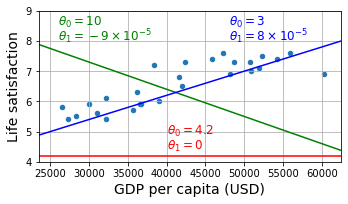
\includegraphics[width=\textwidth,height=0.75\textheight,keepaspectratio]{images/ch01/cell_34_out_0.png}
\end{center}


\end{frame}

\begin{frame}[fragile]{Tải và chuẩn bị dữ liệu Sự hài lòng trong cuộc sống (Biểu đồ) (Biểu đồ) (Tiếp theo 1)}
\begin{lstlisting}[language=Python]
from sklearn import linear_model

X_sample = country_stats[[gdppc_col]].values
y_sample = country_stats[[lifesat_col]].values

lin1 = linear_model.LinearRegression()
lin1.fit(X_sample, y_sample)

t0, t1 = lin1.intercept_[0], lin1.coef_.ravel()[0]
print(f"θ0={t0:.2f}, θ1={t1:.2e}")
\end{lstlisting}


\end{frame}

\begin{frame}[fragile]{Tải và chuẩn bị dữ liệu Sự hài lòng trong cuộc sống (Biểu đồ) (Biểu đồ) (Tiếp theo 2)}
\textbf{Kết quả:}
\begin{verbatim}
θ0=3.75, θ1=6.78e-05
\end{verbatim}


\end{frame}

\begin{frame}[fragile]{Tải và chuẩn bị dữ liệu Sự hài lòng trong cuộc sống (Biểu đồ) (Biểu đồ) (Tiếp theo 3)}
\begin{lstlisting}[language=Python]
country_stats.plot(kind='scatter', figsize=(5, 3), grid=True,
                   x=gdppc_col, y=lifesat_col)

X = np.linspace(min_gdp, max_gdp, 1000)
plt.plot(X, t0 + t1 * X, "b")

plt.text(max_gdp - 20_000, min_life_sat + 1.9,
         fr"$\theta_0 = {t0:.2f}$", color="b")
plt.text(max_gdp - 20_000, min_life_sat + 1.3,
         fr"$\theta_1 = {t1 * 1e5:.2f} \times 10^{{-5}}$", color="b")

plt.axis([min_gdp, max_gdp, min_life_sat, max_life_sat])

save_fig('best_fit_model_plot')
\end{lstlisting}


\end{frame}

\begin{frame}[fragile]{Tải và chuẩn bị dữ liệu Sự hài lòng trong cuộc sống (Biểu đồ) (Biểu đồ) (Tiếp theo 4)}
\begin{lstlisting}[language=Python]
plt.show()
\end{lstlisting}


\end{frame}

\begin{frame}[allowframebreaks]{Tải và chuẩn bị dữ liệu Sự hài lòng trong cuộc sống (Biểu đồ) (Biểu đồ) (Biểu đồ)}
\begin{center}
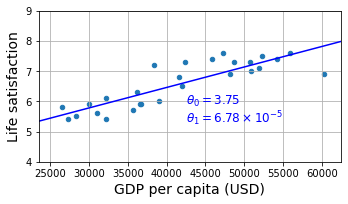
\includegraphics[width=\textwidth,height=0.75\textheight,keepaspectratio]{images/ch01/cell_36_out_0.png}
\end{center}


\end{frame}

\begin{frame}[fragile]{Tải và chuẩn bị dữ liệu Sự hài lòng trong cuộc sống (Biểu đồ) (Biểu đồ) (Biểu đồ) (Tiếp theo 1)}
\begin{lstlisting}[language=Python]
cyprus_gdp_per_capita = gdp_per_capita[gdppc_col].loc["Cyprus"]
cyprus_gdp_per_capita
\end{lstlisting}

\textbf{Kết quả:}
\begin{verbatim}
37655.1803457421
\end{verbatim}

\begin{lstlisting}[language=Python]
cyprus_predicted_life_satisfaction = lin1.predict([[cyprus_gdp_per_capita]])[0, 0]
cyprus_predicted_life_satisfaction
\end{lstlisting}


\end{frame}

\begin{frame}[fragile]{Tải và chuẩn bị dữ liệu Sự hài lòng trong cuộc sống (Biểu đồ) (Biểu đồ) (Biểu đồ) (Tiếp theo 2)}
\textbf{Kết quả:}
\begin{verbatim}
6.301656332738056
\end{verbatim}


\end{frame}

\begin{frame}[fragile]{Tải và chuẩn bị dữ liệu Sự hài lòng trong cuộc sống (Biểu đồ) (Biểu đồ) (Biểu đồ) (Tiếp theo 3)}
\begin{lstlisting}[language=Python]
country_stats.plot(kind='scatter', figsize=(5, 3), grid=True,
                   x=gdppc_col, y=lifesat_col)

X = np.linspace(min_gdp, max_gdp, 1000)
plt.plot(X, t0 + t1 * X, "b")

plt.text(min_gdp + 22_000, max_life_sat - 1.1,
         fr"$\theta_0 = {t0:.2f}$", color="b")
plt.text(min_gdp + 22_000, max_life_sat - 0.6,
         fr"$\theta_1 = {t1 * 1e5:.2f} \times 10^{{-5}}$", color="b")

plt.plot([cyprus_gdp_per_capita, cyprus_gdp_per_capita],
         [min_life_sat, cyprus_predicted_life_satisfaction], "r--")
plt.text(cyprus_gdp_per_capita + 1000, 5.0,
\end{lstlisting}


\end{frame}

\begin{frame}[fragile]{Tải và chuẩn bị dữ liệu Sự hài lòng trong cuộc sống (Biểu đồ) (Biểu đồ) (Biểu đồ) (Tiếp theo 4)}
\begin{lstlisting}[language=Python]
         fr"Prediction = {cyprus_predicted_life_satisfaction:.2f}", color="r")
plt.plot(cyprus_gdp_per_capita, cyprus_predicted_life_satisfaction, "ro")

plt.axis([min_gdp, max_gdp, min_life_sat, max_life_sat])

plt.show()
\end{lstlisting}


\end{frame}

\begin{frame}[allowframebreaks]{Tải và chuẩn bị dữ liệu Sự hài lòng trong cuộc sống (Biểu đồ) (Biểu đồ) (Biểu đồ) (Biểu đồ)}
\begin{center}
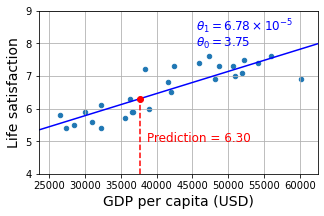
\includegraphics[width=\textwidth,height=0.75\textheight,keepaspectratio]{images/ch01/cell_39_out_0.png}
\end{center}


\end{frame}

\begin{frame}[fragile]{Tải và chuẩn bị dữ liệu Sự hài lòng trong cuộc sống (Biểu đồ) (Biểu đồ) (Biểu đồ) (Biểu đồ) (Tiếp theo 1)}
\begin{lstlisting}[language=Python]
missing_data = full_country_stats[(full_country_stats[gdppc_col] < min_gdp) |
                                  (full_country_stats[gdppc_col] > max_gdp)]
missing_data
\end{lstlisting}


\end{frame}

\begin{frame}[fragile]{Tải và chuẩn bị dữ liệu Sự hài lòng trong cuộc sống (Biểu đồ) (Biểu đồ) (Biểu đồ) (Biểu đồ) (Tiếp theo 2)}
\textbf{Kết quả:}
\begin{verbatim}
GDP per capita (USD)  Life satisfaction
Country                                              
South Africa          11466.189672                4.7
Colombia              13441.492952                6.3
Brazil                14063.982505                6.4
Mexico                17887.750736                6.5
Chile                 23324.524751                6.5
Norway                63585.903514                7.6
Switzerland           68393.306004                7.5
Ireland               89688.956958                7.0
Luxembourg           110261.157353                6.9
\end{verbatim}


\end{frame}

\begin{frame}[fragile]{Tải và chuẩn bị dữ liệu Sự hài lòng trong cuộc sống (Biểu đồ) (Biểu đồ) (Biểu đồ) (Biểu đồ) (Tiếp theo 3)}
\begin{lstlisting}[language=Python]
position_text_missing_countries = {
    "South Africa": (20_000, 4.2),
    "Colombia": (6_000, 8.2),
    "Brazil": (18_000, 7.8),
    "Mexico": (24_000, 7.4),
    "Chile": (30_000, 7.0),
    "Norway": (51_000, 6.2),
    "Switzerland": (62_000, 5.7),
    "Ireland": (81_000, 5.2),
    "Luxembourg": (92_000, 4.7),
}
\end{lstlisting}


\end{frame}

\begin{frame}[fragile]{Tải và chuẩn bị dữ liệu Sự hài lòng trong cuộc sống (Biểu đồ) (Biểu đồ) (Biểu đồ) (Biểu đồ) (Tiếp theo 4)}
\begin{lstlisting}[language=Python]
full_country_stats.plot(kind='scatter', figsize=(8, 3),
                        x=gdppc_col, y=lifesat_col, grid=True)

for country, pos_text in position_text_missing_countries.items():
    pos_data_x, pos_data_y = missing_data.loc[country]
    plt.annotate(country, xy=(pos_data_x, pos_data_y),
                 xytext=pos_text, fontsize=12,
                 arrowprops=dict(facecolor='black', width=0.5,
                                 shrink=0.08, headwidth=5))
    plt.plot(pos_data_x, pos_data_y, "rs")

X = np.linspace(0, 115_000, 1000)
plt.plot(X, t0 + t1 * X, "b:")

\end{lstlisting}


\end{frame}

\begin{frame}[fragile]{Tải và chuẩn bị dữ liệu Sự hài lòng trong cuộc sống (Biểu đồ) (Biểu đồ) (Biểu đồ) (Biểu đồ) (Tiếp theo 5)}
\begin{lstlisting}[language=Python]
lin_reg_full = linear_model.LinearRegression()
Xfull = np.c_[full_country_stats[gdppc_col]]
yfull = np.c_[full_country_stats[lifesat_col]]
lin_reg_full.fit(Xfull, yfull)

t0full, t1full = lin_reg_full.intercept_[0], lin_reg_full.coef_.ravel()[0]
X = np.linspace(0, 115_000, 1000)
plt.plot(X, t0full + t1full * X, "k")

plt.axis([0, 115_000, min_life_sat, max_life_sat])

save_fig('representative_training_data_scatterplot')
plt.show()
\end{lstlisting}


\end{frame}

\begin{frame}[allowframebreaks]{Tải và chuẩn bị dữ liệu Sự hài lòng trong cuộc sống (Biểu đồ) (Biểu đồ) (Biểu đồ) (Biểu đồ) (Biểu đồ)}
\begin{center}
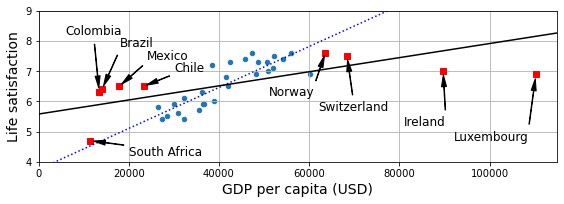
\includegraphics[width=\textwidth,height=0.75\textheight,keepaspectratio]{images/ch01/cell_42_out_0.png}
\end{center}


\end{frame}

\begin{frame}[fragile]{Tải và chuẩn bị dữ liệu Sự hài lòng trong cuộc sống (Biểu đồ) (Biểu đồ) (Biểu đồ) (Biểu đồ) (Biểu đồ) (Tiếp theo 1)}
\begin{lstlisting}[language=Python]
from sklearn import preprocessing
from sklearn import pipeline

full_country_stats.plot(kind='scatter', figsize=(8, 3),
                        x=gdppc_col, y=lifesat_col, grid=True)

poly = preprocessing.PolynomialFeatures(degree=10, include_bias=False)
scaler = preprocessing.StandardScaler()
lin_reg2 = linear_model.LinearRegression()

pipeline_reg = pipeline.Pipeline([
    ('poly', poly),
    ('scal', scaler),
    ('lin', lin_reg2)])
\end{lstlisting}


\end{frame}

\begin{frame}[fragile]{Tải và chuẩn bị dữ liệu Sự hài lòng trong cuộc sống (Biểu đồ) (Biểu đồ) (Biểu đồ) (Biểu đồ) (Biểu đồ) (Tiếp theo 2)}
\begin{lstlisting}[language=Python]
pipeline_reg.fit(Xfull, yfull)
curve = pipeline_reg.predict(X[:, np.newaxis])
plt.plot(X, curve)

plt.axis([0, 115_000, min_life_sat, max_life_sat])

save_fig('overfitting_model_plot')
plt.show()
\end{lstlisting}


\end{frame}

\begin{frame}[allowframebreaks]{Tải và chuẩn bị dữ liệu Sự hài lòng trong cuộc sống (Biểu đồ) (Biểu đồ) (Biểu đồ) (Biểu đồ) (Biểu đồ) (Biểu đồ)}
\begin{center}
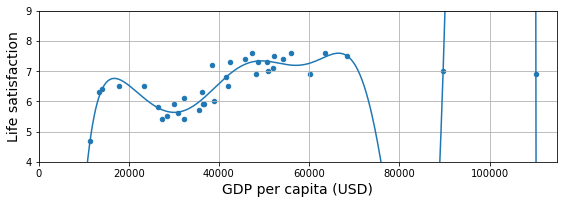
\includegraphics[width=\textwidth,height=0.75\textheight,keepaspectratio]{images/ch01/cell_43_out_0.png}
\end{center}


\end{frame}

\begin{frame}[fragile]{Tải và chuẩn bị dữ liệu Sự hài lòng trong cuộc sống (Biểu đồ) (Biểu đồ) (Biểu đồ) (Biểu đồ) (Biểu đồ) (Biểu đồ) (Tiếp theo 1)}
\begin{lstlisting}[language=Python]
w_countries = [c for c in full_country_stats.index if "W" in c.upper()]
full_country_stats.loc[w_countries][lifesat_col]
\end{lstlisting}

\textbf{Kết quả:}
\begin{verbatim}
Country
New Zealand    7.3
Sweden         7.3
Norway         7.6
Switzerland    7.5
Name: Life satisfaction, dtype: float64
\end{verbatim}


\end{frame}

\begin{frame}[fragile]{Tải và chuẩn bị dữ liệu Sự hài lòng trong cuộc sống (Biểu đồ) (Biểu đồ) (Biểu đồ) (Biểu đồ) (Biểu đồ) (Biểu đồ) (Tiếp theo 2)}
\begin{lstlisting}[language=Python]
all_w_countries = [c for c in gdp_per_capita.index if "W" in c.upper()]
gdp_per_capita.loc[all_w_countries].sort_values(by=gdppc_col)
\end{lstlisting}


\end{frame}

\begin{frame}[fragile]{Tải và chuẩn bị dữ liệu Sự hài lòng trong cuộc sống (Biểu đồ) (Biểu đồ) (Biểu đồ) (Biểu đồ) (Biểu đồ) (Biểu đồ) (Tiếp theo 3)}
\textbf{Kết quả:}
\begin{verbatim}
GDP per capita (USD)
Country                                         
Malawi                               1486.778248
Rwanda                               2098.710362
Zimbabwe                             2744.690758
Africa Western and Central           4003.158913
Papua New Guinea                     4101.218882
Lower middle income                  6722.809932
Eswatini                             8392.717564
Low & middle income                 10293.855325
Arab World                          13753.707307
Botswana                            16040.008473
World                               16194.040310
New Zealand                         42404.393738
Sweden                              50683.323510
... (đã cắt bớt)
\end{verbatim}


\end{frame}

\begin{frame}[fragile]{Tải và chuẩn bị dữ liệu Sự hài lòng trong cuộc sống (Biểu đồ) (Biểu đồ) (Biểu đồ) (Biểu đồ) (Biểu đồ) (Biểu đồ) (Tiếp theo 4)}
\begin{lstlisting}[language=Python]
country_stats.plot(kind='scatter', x=gdppc_col, y=lifesat_col, figsize=(8, 3))
missing_data.plot(kind='scatter', x=gdppc_col, y=lifesat_col,
                  marker="s", color="r", grid=True, ax=plt.gca())

X = np.linspace(0, 115_000, 1000)
plt.plot(X, t0 + t1*X, "b:", label="Linear model on partial data")
plt.plot(X, t0full + t1full * X, "k-", label="Linear model on all data")

ridge = linear_model.Ridge(alpha=10**9.5)
X_sample = country_stats[[gdppc_col]]
y_sample = country_stats[[lifesat_col]]
ridge.fit(X_sample, y_sample)
t0ridge, t1ridge = ridge.intercept_[0], ridge.coef_.ravel()[0]
plt.plot(X, t0ridge + t1ridge * X, "b--",
\end{lstlisting}


\end{frame}

\begin{frame}[fragile]{Tải và chuẩn bị dữ liệu Sự hài lòng trong cuộc sống (Biểu đồ) (Biểu đồ) (Biểu đồ) (Biểu đồ) (Biểu đồ) (Biểu đồ) (Tiếp theo 5)}
\begin{lstlisting}[language=Python]
         label="Regularized linear model on partial data")
plt.legend(loc="lower right")

plt.axis([0, 115_000, min_life_sat, max_life_sat])

save_fig('ridge_model_plot')
plt.show()
\end{lstlisting}


\end{frame}

\begin{frame}[allowframebreaks]{Tải và chuẩn bị dữ liệu Sự hài lòng trong cuộc sống (Biểu đồ) (Biểu đồ) (Biểu đồ) (Biểu đồ) (Biểu đồ) (Biểu đồ) (Biểu đồ)}
\begin{center}
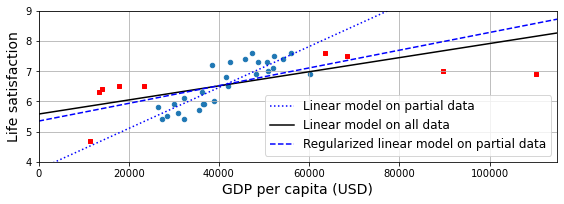
\includegraphics[width=\textwidth,height=0.75\textheight,keepaspectratio]{images/ch01/cell_46_out_0.png}
\end{center}


\end{frame}

\begin{frame}[allowframebreaks]{Giải pháp tập thể dục}
\# Giải pháp tập thể dục


\end{frame}

\begin{frame}[allowframebreaks]{Giải pháp tập thể dục}
1. Machine Learning is about building systems that can learn from data. Learning means getting better at some task, given some performance measure.

2. Machine Learning is great for complex problems for which we have no algorithmic solution, to replace long lists of hand-tuned rules, to build systems that adapt to fluctuating environments, and finally to help humans learn (e.g., data mining).

3. A labeled training set is a training set that contains the desired solution (a.k.a. a label) for each instance.

4. The two most common supervised tasks are regression and classification.

5. Common unsupervised tasks include clustering, visualization, dimensionality reduction, and association rule learning.

6. Reinforcement Learning is likely to perform best if we want a robot to learn to walk in various unknown terrains, since this is typically the type of problem that Reinforcement Learning tackles. It might be possible to express the problem as a supervised or semi-supervised learning problem, but it would be less natural.

7. If you don't know how to define the groups, then you can use a clustering algorithm (unsupervised learning) to segment your customers into clusters of similar customers. However, if you know what groups you would like to have, then you can feed many examples of each group to a classification algorithm (supervised learning), and it will classify all your customers into these groups.

8. Spam detection is a typical supervised learning problem: the algorithm is fed many emails along with their labels (spam or not spam).

9. An online learning system can learn incrementally, as opposed to a batch learning system. This makes it capable of adapting rapidly to both changing data and autonomous systems, and of training on very large quantities of data.

10. Out-of-core algorithms can handle vast quantities of data that cannot fit in a computer's main memory. An out-of-core learning algorithm chops the data into mini-batches and uses online learning techniques to learn from these mini-batches.

11. An instance-based learning system learns the training data by heart; then, when given a new instance, it uses a similarity measure to find the most similar learned instances and uses them to make predictions.

12. A model has one or more model parameters that determine what it will predict given a new instance (e.g., the slope of a linear model). A learning algorithm tries to find optimal values for these parameters such that the model generalizes well to new instances. A hyperparameter is a parameter of the learning algorithm itself, not of the model (e.g., the amount of regularization to apply).

13. Model-based learning algorithms search for an optimal value for the model parameters such that the model will generalize well to new instances. We usually train such systems by minimizing a cost function that measures how bad the system is at making predictions on the training data, plus a penalty for model complexity if the model is regularized. To make predictions, we feed the new instance's features into the model's prediction function, using the parameter values found by the learning algorithm.

14. Some of the main challenges in Machine Learning are the lack of data, poor data quality, nonrepresentative data, uninformative features, excessively simple models that underfit the training data, and excessively complex models that overfit the data.

15. If a model performs great on the training data but generalizes poorly to new instances, the model is likely overfitting the training data (or we got extremely lucky on the training data). Possible solutions to overfitting are getting more data, simplifying the model (selecting a simpler algorithm, reducing the number of parameters or features used, or regularizing the model), or reducing the noise in the training data.

16. A test set is used to estimate the generalization error that a model will make on new instances, before the model is launched in production.

17. A validation set is used to compare models. It makes it possible to select the best model and tune the hyperparameters.

18. The train-dev set is used when there is a risk of mismatch between the training data and the data used in the validation and test datasets (which should always be as close as possible to the data used once the model is in production). The train-dev set is a part of the training set that's held out (the model is not trained on it). The model is trained on the rest of the training set, and evaluated on both the train-dev set and the validation set. If the model performs well on the training set but not on the train-dev set, then the model is likely overfitting the training set. If it performs well on both the training set and the train-dev set, but not on the validation set, then there is probably a significant data mismatch between the training data and the validation + test data, and you should try to improve the training data to make it look more like the validation + test data.

19. If you tune hyperparameters using the test set, you risk overfitting the test set, and the generalization error you measure will be optimistic (you may launch a model that performs worse than you expect).


\end{frame}

\end{document}
